% The methods for implementation of a behavioral, discrete-time PLL simulator and for the PLL loop filter automation and optimization will be covered here.

% \hl{Talk about how simulator is implemented:}
% \hl{Discrete simulation models of phase noise, dco etc}
% \hl{Filter optimization}
% \hl{-phase noise and lock time estimate in frequency domain}


\section{Loop Filter Design Automation}\label{methods_lf_design_approach}
The automation approach for ADPLL loop filter design implemented in this work will be outlined here.

\subsection{Design sequence}
	Design automation for ADPLL loop filter is implemented with a strategy that is illustrated in figure \ref{fig:filt_design_seq}, that utilizes a continuous time-approximation based model of the PLL to generate a loop filter design which minimizes the total integrated phase noise power out of the PLL. The optimized continuous filter then undergoes discrete time conversion and mapping into digital representation of the design. Second order optimization is then applied to the discretized and digitized filter implementation, to minimize effects of quantization error and filter design error due to finite word effects. A discrete-time, behavioral PLL simulator is then used to verify the filter design for proper lock-time, phase noise and stability. The following sections will detail these processes.

	\begin{figure}[htb!]
		\center\fontfamily{\sfdefault}\selectfont
% XCircuit output "filt_design.tex" for LaTeX input from filt_design.ps
\def\putbox#1#2#3#4{\makebox[0.00000in][l]{\makebox[#1][l]{}\raisebox{\baselineskip}[0.00000in][0.00000in]{\raisebox{#2}[0.00000in][0.00000in]{\scalebox{#3}{#4}}}}}
\def\rightbox#1{\makebox[0.00000in][r]{#1}}
\def\centbox#1{\makebox[0.00000in]{#1}}
\def\topbox#1{\raisebox{-0.60\baselineskip}[0.00000in][0.00000in]{#1}}
\def\midbox#1{\raisebox{-0.20\baselineskip}[0.00000in][0.00000in]{#1}}
   \scalebox{1}{
   \normalsize
   \parbox{6.30000in}{
   \includegraphics[scale=0.70000]{./figs/filt_design.pdf}\\
   % translate x=192 y=896 scale 0.38
   \putbox{1.90400in}{2.66700in}{0.96}{$T_{opt}(s)=\underset{T(s)}{\argmin}\int_0^{f_h}\mathcal{L}(\Delta f|T(s))d\Delta f$}%
   \putbox{0.09800in}{2.89800in}{0.96}{\textbf{Optimize continuous PLL closed loop response $T(s)$ for minimum total integrated phase noise.}}%
   \putbox{0.09800in}{3.71700in}{0.96}{\textbf{Specify PLL system parameters.}}%
   \putbox{0.18200in}{3.39500in}{0.84}{Divider ratio}%
   \putbox{1.52600in}{3.54200in}{0.84}{TDC resolution}%
   \putbox{1.55400in}{3.39500in}{0.84}{KDCO}%
   \putbox{0.18200in}{3.54200in}{0.84}{Reference frequency}%
   \putbox{3.57000in}{3.54200in}{0.96}{$S_{\Phi n_{DCO}}(f)$}%
   \putbox{0.12600in}{2.07900in}{0.96}{\textbf{Convert $T_{opt}(s)$ into discretized loop filter design.}}%
   \putbox{0.21700in}{1.90400in}{0.84}{Convert $T_{opt}(s)$ to loop filter $H_{LF}(s)$ based on provided system specifications.}%
   \putbox{0.21700in}{1.75700in}{0.84}{Use s-to-z transformation to convert $H_{LF}(s)$ to the discrete time $H_{LF}(z)$.}%
   \putbox{0.12600in}{1.26700in}{0.96}{\textbf{Second order optimize loop filter digital implementation.}}%
   \putbox{0.21700in}{1.09200in}{0.84}{Convert $H_{LF}(z)$ to direct form I implementation of its difference equation.}%
   \putbox{0.21700in}{0.94500in}{0.84}{Optimize number of bits per word used in digital implementation for quantization noise and filter accuracy.}%
   \putbox{0.12600in}{0.44800in}{0.96}{\textbf{Verify design with simulation.}}%
   \putbox{0.21700in}{0.27300in}{0.84}{Utilize behavioral, discrete event simulator to capture non-linear and discrete time effects.}%
   \putbox{0.21700in}{0.12600in}{0.84}{Monte-Carlo sampling for KDCO. initial frequency error to analyze stability, phase noise and lock time across PVT.}%
   \putbox{2.57600in}{3.54200in}{0.84}{DCO phase noise - }%
   } % close 'parbox'
   } % close 'scalebox'
   \vspace{-\baselineskip} % this is not necessary, but looks better
\fontfamily{\rmdefault}\selectfont

		\caption{Filter design sequence.}
		\label{fig:filt_design_seq}
	\end{figure}
	\FloatBarrier

\subsection{Loop filter Prototype}
	The design automation approach developed utilizes a fixed loop filter as a prototype for all loop filter designs. This choice was derived from several criteria that were establish for desirable ADPLL operation:
	\begin{enumerate}[itemsep=0pt,label=\protect\mycirc{\arabic*}]
		\setlength\itemsep{-0.8em}
		\item Zero steady state phase error, to ensure accuracy of synthesized frequency.
		\item Loop filter output should remain constant if input (phase error) goes to 0.
		\item Minimize complexity of implemented logic, i.e. minimize number of poles and zeros.
		\item Low pass response of PLL in closed-loop.
	\end{enumerate}
	To satisfy criterion 1, the loop filter response must include an integrator (1/s) term in the transfer function \cite{ogata_2010}. A PLL with loop filter containing such an integrator is commonly classified as type II, and sans the integrator is type I \cite{gardner_2005}. A rational starting point is to consider a proportional-integral-derivative (PID) controller \cite{ogata_2010_pid} for the loop filter, whose transfer function is given in equation \ref{eq:pid_controller}. This filter contains coefficients $K_d$, $K_p$, $K_i$ which set the gain of the derivative (s), proportional and integral (1/s) terms respectively. 
	\begin{equation}\label{eq:pid_controller}
		\textnormal{H}_{LF}(s) = sK_d + K_p + \frac{K_i}{s} = \frac{K_d}{s}\left(s^2 + s\frac{K_p}{K_d} + \frac{K_i}{K_d}\right)
	\end{equation}
	Application of the loop filter to the continuous PLL transfer function model from section \ref{cont_pll_tf} produces the PLL loop gain in \ref{pid_pll_loop_gain} and the closed PLL loop response in \ref{eq:pid_pll_tf}.
	\begin{equation} \label{pid_pll_loop_gain}
		\mathrm{L}(s) = \textnormal{H}_{LF}(s)\textnormal{H}_{VCO}(s)\textnormal{H}_{div}(s) = \frac{2\pi K_{VCO}K_d}{\mathrm{N}}\frac{1}{s^2}\left(s^2 + s\frac{K_p}{K_d} + \frac{K_i}{K_d}\right)
	\end{equation}
	\begin{align} \label{eq:pid_pll_tf}
		\mathrm{T}(s) = \frac{\Phi_{out}(s)}{\Phi_{ref}(s)} = \frac{2\pi K_{VCO}\left(s^2K_d + sK_p + K_i\right)}{s^2\left(1 + \frac{2\pi K_{VCO}K_d}{\mathrm{N}}\right) + \frac{2\pi K_{VCO}}{\mathrm{N}}\left(sK_p + K_i\right)} = \mathrm{N}\frac{\mathrm{L}(s)}{1 + \mathrm{L}(s)}
	\end{align}
	It should be noted that in the closed loop configuration, this PLL phase transfer function contains two poles and two zeros. This is not a low pass response as desired per criterion 4, needed for satisfactory PLL phase noise power spectrum as will later be discussed. In order achieve low pass operation, the derivative term $K_d$ must be set to zero, yielding a proportional-integral (PI) controller for the loop filter:
	\begin{align} \label{eq:full_pi_pll_tf}
		\mathrm{T}(s) = \frac{\Phi_{out}(s)}{\Phi_{ref}(s)} = \frac{2\pi K_{VCO}\left(sK_p + K_i\right)}{s^2 + \frac{2\pi K_{VCO}}{\mathrm{N}}\left(sK_p + K_i\right)} = \mathrm{N}\frac{\mathrm{L}(s)}{1 + \mathrm{L}(s)} 
	\end{align}
	Steady state zero phase error can be verified by solving the closed loop $\Phi_e(s)$ for s=0:
	\begin{align}
		\left.\Phi_e(s)\right\vert_{s=0} = \left(\Phi_{ref}(0) - \frac{\Phi_{out}(0)}{\mathrm{N}}\right) = \Phi_{ref}(0)\left(1 - \frac{\Phi_{out}(0)}{\mathrm{N}\Phi_{ref}(0)}\right)= \Phi_{ref}(0)\left(1 - \frac{\mathrm{N}}{\mathrm{N}}\right) = 0
	\end{align}

		\subsubsection{Continuous PI-loop filter design}
			Given a PI-controller loop filter, which can be optionally represented using a pole at zero and a zero with $\omega_z = K_i/K_p$:
			\begin{equation} \label{eq:pi_pll_tf}
				\textnormal{H}_{LF}(s) = K_p + \frac{K_i}{s}  = \frac{K_i}{s}\left(\frac{s}{\omega_z} + 1\right) 
			\end{equation}
			Selection of (not-necessarily optimal) PI controller gains can be easily derived from overall PLL settling time requirements. Suppose that settling time $t_s$ is defined such that the PLL settles within $\pm \delta$ of the final value for a step input. If the initial and final PLL output frequencies are $f_i$ and $Nf_{ref}$, and settling with $\pm f_{tol}$ is desired,  $\delta = f_{tol}/|f_i - Nf_{ref}|$. Setting time is therefore:
			\begin{equation}
				t_s = -\tau\ln(\delta)
			\end{equation}
			Thus, to find settling time, a value for the PLL time constant $\tau$ must be derived. Rewriting equation \ref{eq:full_pi_pll_tf} with substitutions $\omega_z = K_i/K_p$ and $\mathrm{K} = 2\pi K_{VCO}K_i/\mathrm{N}$:
			\begin{equation} \label{eq:simp_pi_pll_tf}
				\frac{\Phi_{out}(s)}{\Phi_{ref}(s)} = \mathrm{N}\cdot\frac{s\frac{K}{\omega_z} + K }{s^2 + s\frac{K}{\omega_z} + K}
			\end{equation}
			If the second order denominator can be redefined in terms of a natural frequency $\omega_n$ and damping $\zeta$, such that:
			\begin{equation}
				s^2 + s\frac{K}{\omega_z} + K = s^2 + s2\zeta\omega_n + \omega_n^2
			\end{equation}
			It is then found that $\omega_n = \sqrt{K}$, and $\omega_z = \sqrt{K}/2\zeta$. The poles of equation \ref{eq:simp_pi_pll_tf} are then located at s = $\zeta\sqrt{K} \pm \sqrt{K}\sqrt{1-\zeta^2}$.
			The settling time of the PLL will be determined by the real portion of dominant pole of equation \ref{eq:simp_pi_pll_tf}, specifically $\tau = 1/|\min(\Re(\{s_{p1}, s_{p2}\}))|$. Based on the pole-zero plot of figure \ref{fig:pi_pll_pz}, it can be observed that the dominant pole location is maximized with $\zeta=1$. The pole-zero loci orientations are based on increasing $\zeta$ values. According to Razavi \cite{razavi_2017}, $\zeta$ is usually 
			"chosen to be $>\sqrt{2}/2$ or even 1 to avoid excessive ringing."
			\begin{figure}[htb!]
				\center\fontfamily{\sfdefault}\selectfont
% XCircuit output "pi_pz_plot.tex" for LaTeX input from pi_pz_plot.ps
\def\putbox#1#2#3#4{\makebox[0.00000in][l]{\makebox[#1][l]{}\raisebox{\baselineskip}[0.00000in][0.00000in]{\raisebox{#2}[0.00000in][0.00000in]{\scalebox{#3}{#4}}}}}
\def\rightbox#1{\makebox[0.00000in][r]{#1}}
\def\centbox#1{\makebox[0.00000in]{#1}}
\def\topbox#1{\raisebox{-0.60\baselineskip}[0.00000in][0.00000in]{#1}}
\def\midbox#1{\raisebox{-0.20\baselineskip}[0.00000in][0.00000in]{#1}}
   \scalebox{1}{
   \normalsize
   \parbox{4.20000in}{
   \includegraphics[scale=0.70000]{./figs/pi_pz_plot.pdf}\\
   % translate x=800 y=416 scale 0.38
   \putbox{2.85600in}{0.67900in}{1.20}{$\Re(s)$}%
   \putbox{2.30300in}{1.52600in}{1.20}{$\Im(s)$}%
   \putbox{1.89000in}{0.21700in}{1.20}{$\sqrt{\mathrm{K}}$}%
   \putbox{1.45600in}{1.36500in}{1.20}{$\zeta\sqrt{\mathrm{K}}$}%
   \putbox{2.38700in}{0.95900in}{1.20}{$\sqrt{\mathrm{K}}/2\zeta$}%
   } % close 'parbox'
   } % close 'scalebox'
   \vspace{-\baselineskip} % this is not necessary, but looks better
\fontfamily{\rmdefault}\selectfont

				\caption{PI-controller PLL pole-zero locations.}
				\label{fig:pi_pll_pz}
			\end{figure}
			\FloatBarrier
			To illustrate the effect of the damping coefficient $\zeta$, figure \ref{fig:pi_pll_response} illustrates the example frequency and step responses of a PI-controlled PLL with N=1. Notice excessive peaking and ringing for $\zeta<\sqrt{2}/2$. The peaking observed in the frequency response is unavoidable with the PI-PLL due to the inherent zero in the transfer function. Its effect can be reduced with large $\zeta$, however this will increase PLL settling time. 
			\begin{figure}[htb!]
				\center\includegraphics[width=1.0\textwidth, angle=0]{figs/pi_pll_response.pdf}
				\caption{Example PI-PLL responses with varied $\zeta$.}
				\label{fig:pi_pll_response}
			\end{figure}
			\FloatBarrier
			If $\zeta$ is constrained to $\leq 1$:
			\begin{equation}
				\tau = \frac{1}{|\min(\Re(\{s_{p1}, s_{p2}\}))|} = \frac{1}{\zeta\sqrt{K}}
			\end{equation}
			Thus:
			\begin{equation}
				t_s = \frac{-\ln(\delta)}{\zeta\sqrt{K}} = \frac{-\ln\left(\frac{f_{tol}}{|f_i - Nf_{ref}|}\right)}{\zeta\sqrt{K}} 
			\end{equation}
			Based on specification for settling time and damping $\zeta$, the values for K and $\omega_z$ can be determined. If $K_{VCO}$ and $\mathrm{N}$ are also specified, the PI gain coefficients can be solved additionally.
			\begin{align}
				\omega_z &= \frac{-\ln(\delta)}{2t_s} =  \frac{-\ln\left(\frac{f_{tol}}{|f_i - Nf_{ref}|}\right)}{2t_s}\\
				K &= \frac{\ln^2(\delta)}{\zeta^2t_s^2} =  \frac{\ln^2\left(\frac{f_{tol}}{|f_i - Nf_{ref}|}\right)}{\zeta^2t_s^2}\\
				K_i & = \frac{\mathrm{N}\mathrm{K}}{2\pi K_{VCO}} \\
				K_p & = \frac{K_i}{\omega_z}
			\end{align}

		\subsubsection{PI-controller peaking compensation}
			 To compensate for closed loop peaking, the original PI-controller loop filter of equation \ref{eq:pi_pll_tf} can be modified with the addition of a single tunable pole at $\omega_p$. The closed loop response becomes third order, which complicates direct analysis and design of the loop filter, but can be handled utilizing the numerical optimization approach described in this work.
			\begin{equation} \label{eq:pi_compensated_tf}
				\textnormal{H}_{LF}(s) = \frac{K_i}{s}\frac{\left(\frac{s}{\omega_z} + 1\right)}{\left(\frac{s}{\omega_p} + 1\right)}
			\end{equation}

		\subsubsection{Alternative PID controller permutations} \label{other_pid}
			If individual terms within the PID-controller are dropped, different controller permutations (PD, ID, PI, P, I, D) can be achieved. As mentioned before, inclusion of an integral term is needed to ensure the desired zero steady state error for a PLL, and the derivative term must be removed to achieve low pass response in the PLL. This leaves integral term only controller as the remaining cantidate for PID controller design. Thus, setting the $K_p$ and $K_d$ terms of equation \ref{eq:pid_pll_tf} to zero yields:
			\begin{equation}
				\frac{\Phi_{out}(s)}{\Phi_{ref}(s)} = \frac{2\pi K_{VCO}K_i}{s^2 + \frac{2\pi K_{VCO}}{\mathrm{N}}K_i}
			\end{equation}
			This closed loop transfer function results in a pair of poles at $\pm\sqrt{2\pi K_{VCO}K_i/\mathrm{N}}$. This is not stable, as it can only be manifested as (1) a pair of poles on the imaginary axis, which is an oscillator, or (2) a real pole in the right-half plane and a real pole in the left-half plane, the former of which is not causally stable. Thus a PI-controller is the only viable PID-controller permutation for use in a PLL loop filter. 


	\subsubsection{Discretized Loop Filter Prototype}
		Using the continuous filter discretization approach described in section \ref{lf-discretization} on the loop filter of equation \ref{eq:pi_compensated_tf} results in equation \ref{eq:z_lf}.
		\begin{align}
			\textnormal{H}_{LF}(z) & = \left.\frac{K_i}{s}\frac{\left(\frac{s}{\omega_z} + 1\right)}{\left(\frac{s}{\omega_p} + 1\right)}\right\vert_{s=\frac{1}{\Delta T_s}(1-z^{-1})}
			&= k_i\Delta T_s\frac{\omega_p}{\omega_z}\frac{(1+\omega_z\Delta T_s)-z^{-1}}{(1+\omega_p\Delta T_s) - z^{-1}(2+\omega_p\Delta T_s) + z^{-2}}\label{eq:z_lf}
		\end{align}

		The transformation of \ref{eq:z_lf} into a digitally implementable design as a direct form 1 IIR filter shown in figure \ref{fig:filt_imple}. Its filter coefficients given by equations \ref{eq:a1}-\ref{eq:b1}.
		\begin{figure}[htb!]
			\center\fontfamily{\sfdefault}\selectfont
% XCircuit output "filter_arch_tex.tex" for LaTeX input from filter_arch_tex.ps
\def\putbox#1#2#3#4{\makebox[0.00000in][l]{\makebox[#1][l]{}\raisebox{\baselineskip}[0.00000in][0.00000in]{\raisebox{#2}[0.00000in][0.00000in]{\scalebox{#3}{#4}}}}}
\def\rightbox#1{\makebox[0.00000in][r]{#1}}
\def\centbox#1{\makebox[0.00000in]{#1}}
\def\topbox#1{\raisebox{-0.60\baselineskip}[0.00000in][0.00000in]{#1}}
\def\midbox#1{\raisebox{-0.20\baselineskip}[0.00000in][0.00000in]{#1}}
   \scalebox{1}{
   \normalsize
   \parbox{5.54167in}{
   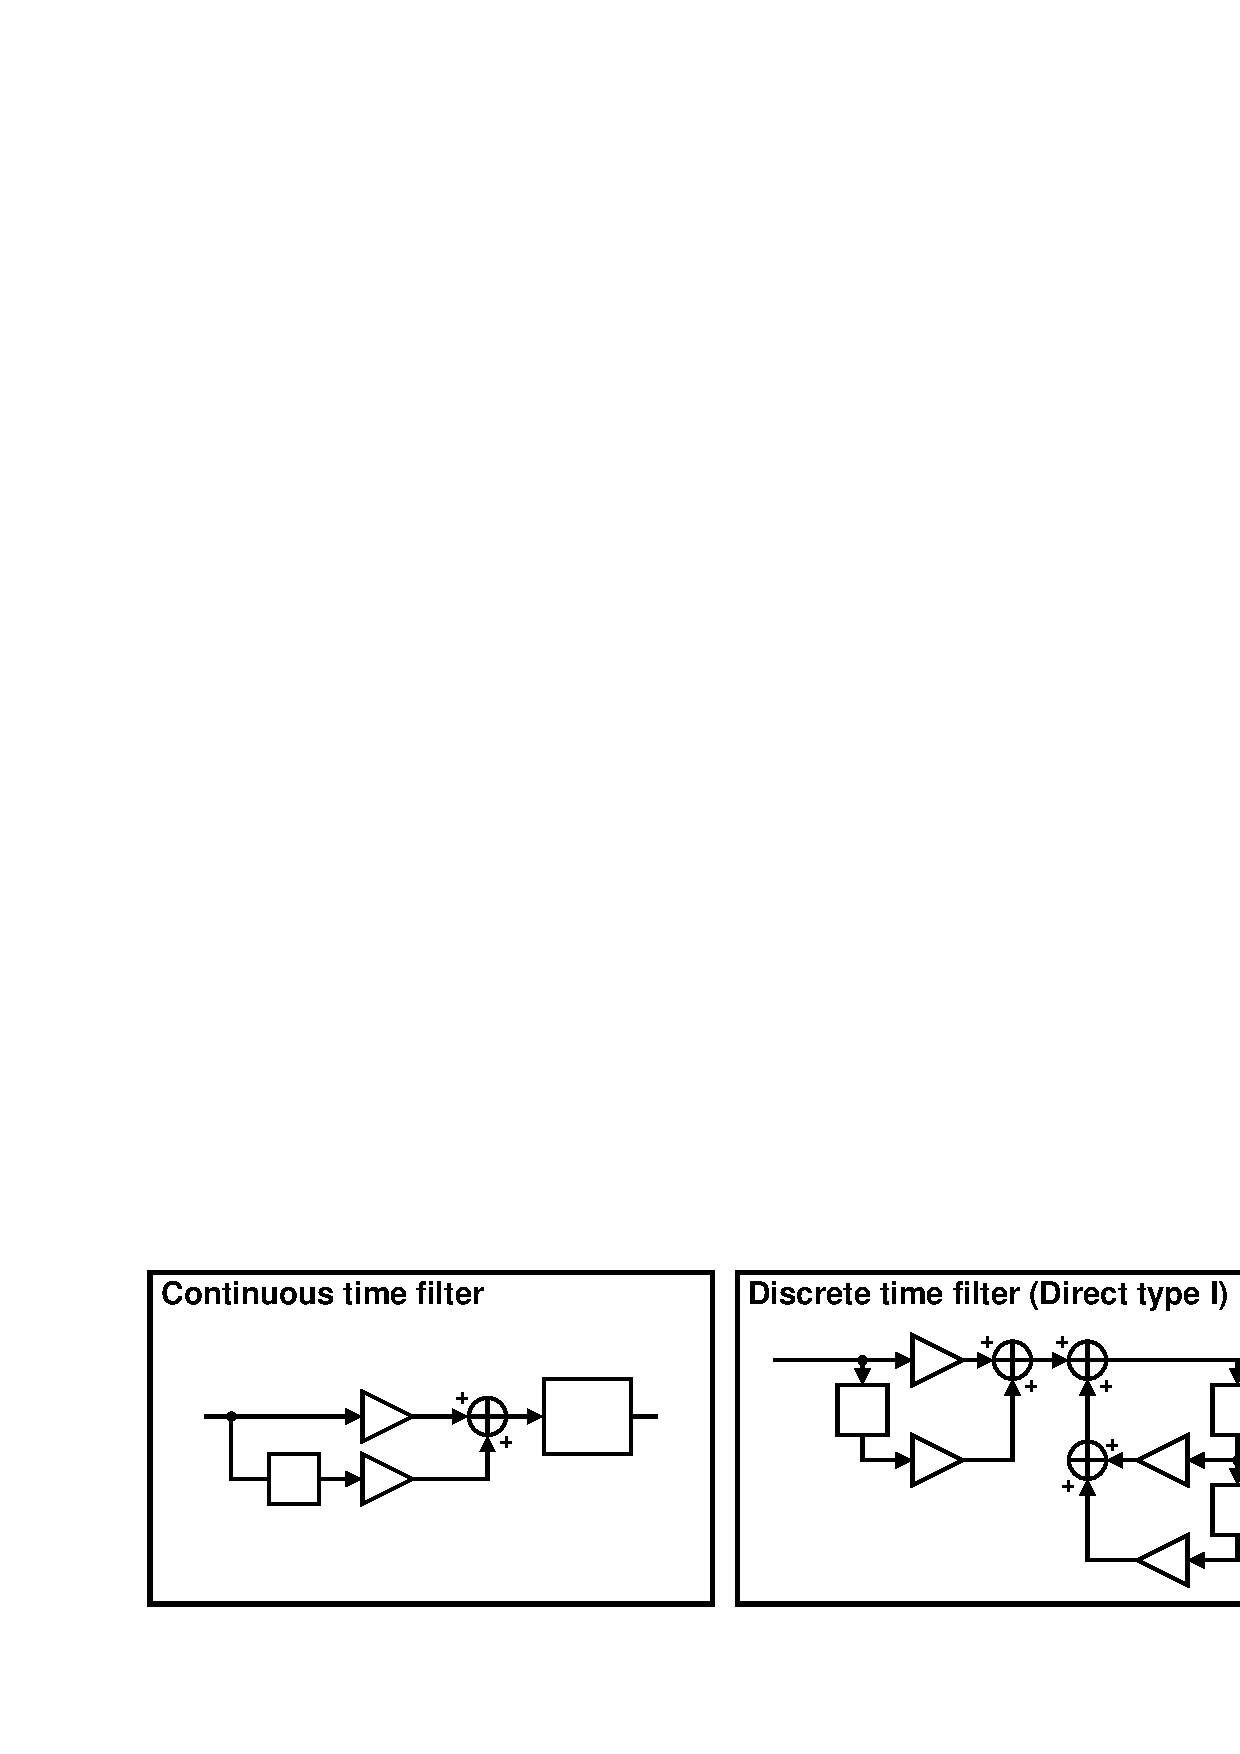
\includegraphics[scale=0.70000]{./figs/filter_arch_tex.pdf}\\
   % translate x=1728 y=944 scale 0.38
   \putbox{1.91800in}{0.90300in}{0.96}{$\frac{1}{\frac{s}{\omega_p} + 1}$}%
   \putbox{1.14800in}{1.01500in}{0.96}{$K_p$}%
   \putbox{1.14800in}{0.72800in}{0.96}{$K_i$}%
   \putbox{0.60900in}{0.58100in}{0.96}{$1/s$}%
   \putbox{0.25900in}{0.98700in}{0.96}{x[n]}%
   \putbox{2.35900in}{0.98700in}{0.96}{y[n]}%
   \putbox{2.92600in}{1.25300in}{0.96}{x[n]}%
   \putbox{5.17300in}{1.16200in}{0.96}{y[n]}%
   \putbox{3.26200in}{0.90300in}{0.96}{$z^{-1}$}%
   \putbox{3.73100in}{1.28100in}{0.96}{b$_0$}%
   \putbox{3.73100in}{0.81200in}{0.96}{b$_1$}%
   \putbox{5.01200in}{0.90300in}{0.96}{$z^{-1}$}%
   \putbox{5.01200in}{0.43400in}{0.96}{$z^{-1}$}%
   \putbox{4.60600in}{0.82600in}{0.96}{-a$_1$}%
   \putbox{4.59200in}{0.35700in}{0.96}{-a$_2$}%
   \putbox{5.17300in}{0.69300in}{0.96}{y[n-1]}%
   \putbox{5.15900in}{0.23100in}{0.96}{y[n-2]}%
   } % close 'parbox'
   } % close 'scalebox'
   \vspace{-\baselineskip} % this is not necessary, but looks better
\fontfamily{\rmdefault}\selectfont

			\caption{Implementation of filter.}
			\label{fig:filt_imple}
		\end{figure}
					% y[n] = x[n]\frac{K_i\omega_pT}{\omega_z}\frac{1+\omega_zT}{1+\omega_pT} - x[n-1]\frac{K_i\omega_pT}{\omega_z}\frac{1}{1+\omega_pT} + y[n-1]\frac{2+\omega_pT}{1+\omega_pT} - y[n-2]\frac{1}{1+\omega_pT}\\
					% = a_0x[n] + a_1x[n-1] - b_1y[n-1] - b_2x[n-2] 
		\begin{align}
			a_1 &= -\frac{2+\omega_p\Delta T_s}{1+\omega_p\Delta T_s}\label{eq:a1} 
			& a_2 &= \frac{1}{1+\omega_p\Delta T_s} \\
			b_0 &= \frac{K_i\omega_p\Delta T_s}{\omega_z}\frac{1+\omega_z\Delta T_s}{1+\omega_p\Delta T_s}
			& b_1 &= \frac{K_i\omega_p\Delta T_s}{\omega_z}\frac{1}{1+\omega_p\Delta T_s}\label{eq:b1}
		\end{align}

		%%%%

		\subsubsection{Prototype PLL response}
		Based on the prototype loop filter developed, the PLL closed loop response is developed for usage in the loop optimizer discussed in this work. Applying the discrete-time PLL transfer function model developed in section \ref{discrete_pll_tf}, the PLL loop gain is in equation \ref{eq:z_loop_gain_pi_comp}, and the closed loop transfer function of the PLL is in \ref{eq:z_cl_tf_pi_comp_pll}.
		\begin{align}
			\mathrm{L}(z) &= \mathrm{H}_{TDC}(z)\mathrm{H}_{LF}(z)\mathrm{H}_{DCO}(z)\mathrm{H}_{DIV}(z) \\
			&= 2\pi K_{DCO}K_i\Delta T_s^2\frac{\mathrm{M}}{\mathrm{N}}\frac{\omega_p}{\omega_z}\frac{(1+\omega_z\Delta T_s)-z^{-1}}{(1+\omega_p\Delta T_s) - z^{-1}(3+2\omega_p\Delta T_s) + z^{-2}(3+\omega_p\Delta T_s) - z^{-3}}\label{eq:z_loop_gain_pi_comp}
		\end{align}
		The closed loop z-domain PLL phase transfer function is:
		\begin{align}\label{eq:z_cl_tf_pi_comp_pll}
			\mathrm{T}(z) = \frac{\Phi_{out}(z)}{\Phi_{ref}(z)} &= \frac{2\pi K_{DCO}K_i\Delta T_s^2\mathrm{M}\frac{\omega_p}{\omega_z}(1+\omega_z\Delta T_s)-z^{-1}}{\left(\parbox{4.2in}{$(1+\omega_p\Delta T_s + 2\pi K_{DCO}K_i\Delta T_s^2\frac{\mathrm{M}}{\mathrm{N}}\frac{\omega_p}{\omega_z}(1+\omega_z\Delta T_s))- z^{-1}(3+2\omega_p\Delta T_s+2\pi K_{DCO}K_i\Delta T_s^2\frac{\mathrm{M}}{\mathrm{N}}\frac{\omega_p}{\omega_z})+ z^{-2}(3+\omega_p\Delta T_s) - z^{-3}$}\right)}%\\
			%&= \mathrm{N}\frac{\mathrm{L}(z)}{1+\mathrm{L}(z)}\\
		\end{align}
		Applying z-to-s domain transformation, the continuous s-domain approximation of the loop gain is given in equation \ref{eq:s_loop_gain_pi_comp}, and the closed loop transfer function in equation \ref{eq:s_cl_tf_pi_comp_pll}.
		\begin{align}
			\mathrm{L}(s) = \mathrm{H}_{TDC}(s)\mathrm{H}_{LF}(s)\mathrm{H}_{DCO}(s)\mathrm{H}_{DIV}(s) = \frac{\mathrm{M}}{\mathrm{N}}\frac{K_{DCO}K_i}{s^2} \frac{\left(\frac{s}{\omega_z} + 1\right)}{\left(\frac{s}{\omega_p} + 1\right)}\label{eq:s_loop_gain_pi_comp}
		\end{align}
		\begin{align}\label{eq:s_cl_tf_pi_comp_pll}
			\mathrm{T}(s)=\frac{\Phi_{out}(s)}{\Phi_{ref}(s)} = \frac{\mathrm{M}K_{DCO}K_i\left(\frac{s}{\omega_z} + 1\right)}{s^3\frac{1}{\omega_z} + s^2 + \frac{\mathrm{M}}{\mathrm{N}}K_{DCO}K_i\left(\frac{s}{\omega_z} + 1\right)} = \mathrm{N}\frac{\mathrm{L}(s)}{1+\mathrm{L}(s)} 
		\end{align}



%%%%%%%%%%%%%%%%%%%%%%%%%%%%%%%%%%%%%%%%%%%%%%%%%%%%%%%%%%%%%%%%%%%%
\pagebreak
\section{Behavioral ADPLL simulation}
To fully capture the effects of a discrete time PLL with digital quantization effects, the implementation a behavioral, discrete event PLL simulator is described in the following. The simulator utilizes behavioral models to describe the individual components which comprise the PLL. These components are (1) a clock reference, (2) a TDC, (3) a loop filter, (4) a DCO, and (5) a divider. These behavioral models fully encapsulate effects of time-quantization and digitization. The simulator operates by iterating in fixed time steps of $\Delta t$=1/\texttt{fs}, where each node in the PLL is updated based upon the previous node values in a manner that is defined by each PLL component behavioral model. Each behavioral model is represented programmatically utilizing classes. In simulation, each component instance is represented by a object instance of the respective model class, constructed with any initial parameters (such as division ratio) that describe the component.
\subsection{Simulation engine}
The simulator engine for this work follows the sequence illustrated in figure \ref{fig:simulator} for running a simulation. Given specifications for simulation conditions (listed in the figure), the simulator accordingly initializes model objects that constitute the PLL components in simulation space. Then the simulation is run by entering a simulation loop. 
\begin{figure}[htb!]
	\center\fontfamily{\sfdefault}\selectfont
% XCircuit output "simulator.tex" for LaTeX input from simulator.ps
\def\putbox#1#2#3#4{\makebox[0.00000in][l]{\makebox[#1][l]{}\raisebox{\baselineskip}[0.00000in][0.00000in]{\raisebox{#2}[0.00000in][0.00000in]{\scalebox{#3}{#4}}}}}
\def\rightbox#1{\makebox[0.00000in][r]{#1}}
\def\centbox#1{\makebox[0.00000in]{#1}}
\def\topbox#1{\raisebox{-0.60\baselineskip}[0.00000in][0.00000in]{#1}}
\def\midbox#1{\raisebox{-0.20\baselineskip}[0.00000in][0.00000in]{#1}}
   \scalebox{1}{
   \normalsize
   \parbox{6.25002in}{
   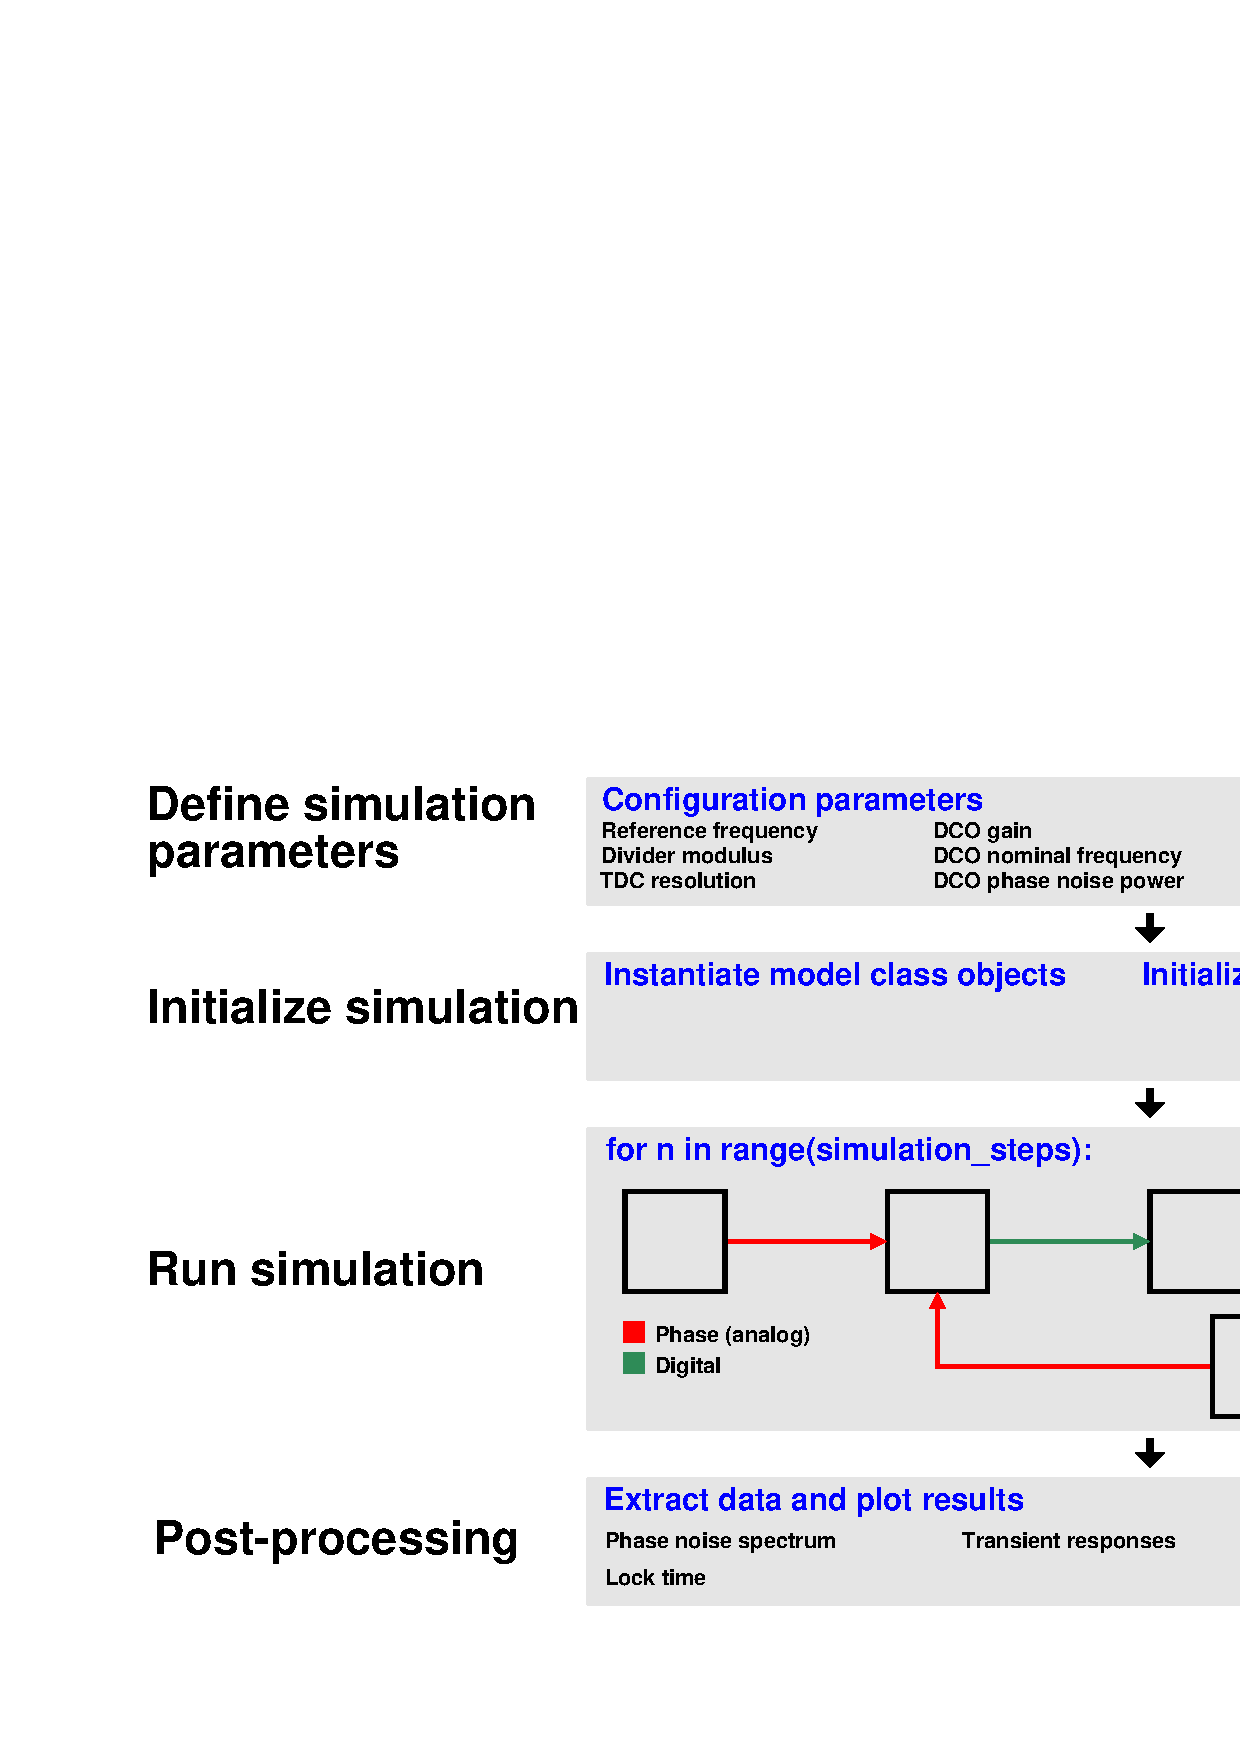
\includegraphics[scale=0.60000]{./figs/simulator.pdf}\\
   % translate x=1040 y=384 scale 0.38
   \putbox{3.08400in}{1.45800in}{0.84}{\texttt{tdc}}%
   \putbox{4.38600in}{0.96000in}{0.84}{\texttt{div}}%
   \putbox{4.15800in}{1.45800in}{0.84}{\texttt{lf}}%
   \putbox{5.18400in}{1.45800in}{0.84}{\texttt{dco}}%
   \putbox{2.03400in}{1.45800in}{0.84}{\texttt{clk}}%
   \putbox{3.48600in}{1.03200in}{0.84}{\texttt{div\_sig[n]}}%
   \putbox{2.38200in}{1.56000in}{0.84}{\texttt{clk\_sig[n]}}%
   \putbox{3.43200in}{1.53600in}{0.84}{\texttt{tdc\_sig[n]}}%
   \putbox{4.48200in}{1.53600in}{0.84}{\texttt{lf\_sig[n]}}%
   \putbox{5.53200in}{1.53600in}{0.84}{\texttt{dco\_sig[n]}}%
   \putbox{4.00800in}{2.35800in}{0.84}{\texttt{clk\_sig[n]}}%
   \putbox{4.00800in}{2.20800in}{0.84}{\texttt{tdc\_sig[n]}}%
   \putbox{4.71000in}{2.35800in}{0.84}{\texttt{lf\_sig[n]}}%
   \putbox{4.71000in}{2.20800in}{0.84}{\texttt{dco\_sig[n]}}%
   \putbox{5.38200in}{2.35800in}{0.84}{\texttt{div\_sig[n]}}%
   \putbox{1.86000in}{2.35800in}{0.84}{\texttt{clk}}%
   \putbox{1.86000in}{2.20800in}{0.84}{\texttt{tdc}}%
   \putbox{2.40600in}{2.35800in}{0.84}{\texttt{lf}}%
   \putbox{2.40600in}{2.20800in}{0.84}{\texttt{dco}}%
   \putbox{2.95800in}{2.35800in}{0.84}{\texttt{div}}%
   \putbox{1.88400in}{0.83400in}{0.84}{t$_{sim}$ = \texttt{n}$\Delta$t}%
   } % close 'parbox'
   } % close 'scalebox'
   \vspace{-\baselineskip} % this is not necessary, but looks better
\fontfamily{\rmdefault}\selectfont

	\caption{Simulation process.}
	\label{fig:simulator}
\end{figure}
\FloatBarrier
The discrete event simulator loop is given in the following pseudocode of listing \ref{sim_code}, with component model objects \{\texttt{clk, tdc, lf, dco, div}\}, and simulation data arrays \{\texttt{clk\_sig, tdc\_sig, lf\_sig, dco\_sig, div\_sig}\}. The simulation operates with a fixed, discrete time step. Each model object is updated at each simulation step (loop iteration) utilizing the class method \texttt{update}, passing any relevant simulation data as arguments to the method. The output state of each component is saved into the respective array instance for each simulation step. 

\begin{lstlisting}[language={Python}, caption={PLL simulation loop Python pseudocode}, label={sim_code}]
for n in range(simulation_steps):
    clk_sig[n] = clk.update()
    tdc_sig[n] = tdc.update(clk_sig[n-1], div_sig[n-1]))
    lf_sig[n]  = lf.update(tdc_sig[n-1], clk_sig[n-1]) #loop filter
    osc_sig[n] = dco.update(lf_sig[n-1])
    div_sig[n] = div.update(osc_sig[n-1], div_n)
    \end{lstlisting}
After the simulation loop reaches completion, the results stored in the simulation data arrays can be post-processed to extract phase noise data, transient behavior and lock time. The following sections will discuss in more detail the implemented behavioral model classes and post-processing.

\subsection{Clock behavioral model}
An ideal behavioral clock model is utilized, given in the pseudocode of listing \ref{clk_code}. The model is instantiated with the clock frequency \texttt{f} and the simulator time step \texttt{dt}. The model incrementing its phase every simulation step by a fixed amount $\Delta \Phi$ = $2\pi$\texttt{f}$\cdot$\texttt{dt}, as in \ref{eq:clk_behavioral_model}. The model outputs an analog phase signal.
\begin{equation}\label{eq:clk_behavioral_model}
	\Phi_{clk}[n] = \Phi_{clk}[n-1] + 2\pi\mathtt{f}\cdot\mathtt{dt}
\end{equation}

\begin{lstlisting}[language={Python}, caption={Ideal clock behavioral model.}, label={clk_code}]
class Clock:
	def __init__(self, f, dt):
		self.f = f 			# clock frequency
		self.dt = dt 		# simulation time step
		self.phase = 0.0	# clock phase state variable

	def update(self):
		self.phase += 2*pi*self.f*self.dt 	# increment phase
		return self.phase
    \end{lstlisting}

\subsection{TDC behavioral model}
The TDC behavioral model takes two analog inputs \texttt{x} and \texttt{y} that are in units of phase, and outputs a digital word that quantifies the phase separation of the signals. The model is instantiated with a resolution parameter \texttt{tdc\_steps}, which defines the number of phase steps per cycle of the reference input \texttt{x} the TDC can resolve. The method \texttt{round} quantizes an floating point argument to the nearest integer.
\begin{equation}
	\text{out}[n] = \left\lfloor0.5 + \mathtt{tdc\_steps}\frac{\mathtt{x}[n]-\mathtt{y}[n]}{2\pi} \right\rfloor
\end{equation}

\begin{lstlisting}[language={Python}, caption={TDC behavioral model.}, label={tdc_code}]
class TDC:
	def __init__(self, tdc_steps):
		self.tdc_steps = tdc_steps

	def update(x, y):
		ph_error = wrap(x-y) 	# wraps phase to be within [0, 2*pi]
		return round(self.tdc_steps*(ph_error/(2*pi)))
\end{lstlisting}
\subsection{Loop filter behavioral model}
The loop filter model implements a discrete-time filter via difference equation that operates on input \texttt{x}. The equivalent of one pole and two zeros are modelled, described using the filter coefficients $\{a_1, a_2; b_0, b_1\}$:
\begin{equation}
\text{H}_{LF}(z) = \frac{b_0 + b_1z^{-1}}{a_0 + a_1z^{-1} + a_2z^{-2}}
\end{equation}
\begin{equation}
\text{y}[n] = -a_1 \text{y}[n-1]-a_2 \text{y}[n-2] + b_0\text{x}[n] + b_1\text{x}[n-1]
\end{equation}
Pseudocode for implementation of the model class is as follows. Data is to be represented with fixed point format, with number of fractional bits \texttt{frac\_bits} and number of integer bits \texttt{int\_bits}. The method \texttt{fixed\_point} rounds floating point values to be equivalent to the nearest representation in the desired fixed point format. The filter coefficients are assumed to be pre-converted to the desired fixed-point equivalent values, and input \texttt{x} is assumed to be integer-valued.
\begin{lstlisting}[language={Python}, caption={Loop filter behavioral model.}, label={lf_code}]
class LoopFilter:
	def __init__(self, a1, a2, b0, b1, int_bits, frac_bits):
		self.a1 = a1;	self.a2 = a2
		self.b0 = b0;	self.b1 = b1
		self.xprev1 = 0;	
		self.yprev1 = 0; self.yprev2 = 0
		self.int_bits=int_bits;	self.frac_bits=frac_bits

	def update(x):
		ynew = -self.a1*self.yprev1 - self.a2*self.yprev2 \\
			   + self.b0*x + self.b1*self.xprev1	# difference equation
		self.yprev2 = self.yprev1	
		self.yprev1 = fixed_point(ynew, self.int_bits, self.frac_bits)
		self.xprev1 = x
		return round(self.yprev1)	# convert to integer
\end{lstlisting}

\subsection{DCO behavioral model}
The DCO is modeled similar to the clock model, with the inclusion of a digital input \texttt{otw} for tuning the frequency. Nominal oscillator frequency is given by \texttt{f0}, and the DCO gain in Hz/LSB of \texttt{otw} is \texttt{kdco}. Additionally, modeling of the $\propto f^-2$ oscillator phase noise component, which is equivalent to random phase walk \cite{vannicola_varshney_1983}, is included utilizing additive random phase walk. Random walk is implemented by stochastically either adding or subtracting a fixed magnitude random walk phase increment $\texttt{krw}$ to the oscillator phase every simulation step. The sign of \texttt{krw} is randomly chosen with equal probability for positive and negative (sampling a bi-delta distribution), implemented with the method \texttt{choice}.
\begin{equation}\label{eq:clk_behavioral_model}
	\Phi_{osc}[n] = \Phi_{osc}[n-1] + 2\pi(\mathtt{f0}+\mathtt{otw}\cdot\mathtt{kdco})\cdot\mathtt{dt} \pm \mathtt{krw}
\end{equation}
\begin{lstlisting}[language={Python}, caption={DCO behavioral model.}, label={dco_code}]
class DCO:
	def __init__(self, f0, kdco, krw, dt):
		self.f0 = f0		# nominal frequency
		self.kdco = kdco 	# DCO gain
		self.krw			# random phase walk gain
		self.dt 			# simulation time step size
		self.phase = 0		# phase state variable

	def update(otw):
		self.phase += 2*pi*(self.f0 + otw*self.kdco)*self.dt + krw*choice([-1,1])
		return self.phase
   \end{lstlisting}

Selection of the parameter \texttt{krw} to achieve a target phase noise level $\mathcal{L}(\Delta f)$ at offset $\Delta f$ from the carrier is as follows.
\begin{figure}[htb!]
	\center\fontfamily{\sfdefault}\selectfont
% XCircuit output "rw_pn.tex" for LaTeX input from rw_pn.ps
\def\putbox#1#2#3#4{\makebox[0.00000in][l]{\makebox[#1][l]{}\raisebox{\baselineskip}[0.00000in][0.00000in]{\raisebox{#2}[0.00000in][0.00000in]{\scalebox{#3}{#4}}}}}
\def\rightbox#1{\makebox[0.00000in][r]{#1}}
\def\centbox#1{\makebox[0.00000in]{#1}}
\def\topbox#1{\raisebox{-0.60\baselineskip}[0.00000in][0.00000in]{#1}}
\def\midbox#1{\raisebox{-0.20\baselineskip}[0.00000in][0.00000in]{#1}}
   \scalebox{1}{
   \normalsize
   \parbox{2.66666in}{
   \includegraphics[scale=0.80000]{./figs/rw_pn.pdf}\\
   % translate x=924 y=776 scale 0.38
   \putbox{0.51200in}{0.71200in}{0.96}{w[n]}%
   \putbox{2.49600in}{0.72800in}{0.96}{y[n]}%
   \putbox{0.96000in}{0.79200in}{0.96}{\texttt{krw}}%
   \putbox{2.11200in}{0.32800in}{0.96}{$z^{-1}$}%
   \putbox{0.04800in}{0.51200in}{0.72}{...,+1,-1,-1,+1,...}%
   \putbox{1.83200in}{0.86400in}{0.96}{Integrator}%
   \putbox{1.19200in}{0.71200in}{0.96}{x[n]}%
   } % close 'parbox'
   } % close 'scalebox'
   \vspace{-\baselineskip} % this is not necessary, but looks better
\fontfamily{\rmdefault}\selectfont

	\caption{Discrete model for oscillator random walk.}
	\label{fig:rw_pn}
\end{figure}
\FloatBarrier
The random walk process described in the behavioral model is represented in figure \ref{fig:rw_pn}, where a random white-spectrum input sequence $w$[n] taking on values $\pm$ 1 with equal probability are multiplied by gain \texttt{krw}, yielding signal $x$[n] that is passed a discrete integrator. The output $y$[n] is then the phase noise signal that is summed with the oscillator phase trajectory. If the simulation is limited to \texttt{sim\_steps} samples, Parseval's theorem for the discrete Fourier transform (DFT) in \ref{eq:parsevals} results in the estimate of the power of x[n] ($\sigma_x^2$) in \ref{eq:white_noise_pow}.
\begin{equation}\label{eq:parsevals}
\sum _{n=0}^{\mathtt{sim\_steps}-1}|\texttt{krw}\cdot w[n]|^{2}=\sum _{k=0}^{\mathtt{sim\_steps}-1}| X[k]|^{2}
\end{equation}
\begin{equation}\label{eq:white_noise_pow}
\sigma_x^2 = |X[k]|^{2} =\texttt{krw}^2
\end{equation}

Computation of the spectrum of the output $y[n]$ of figure \ref{fig:rw_pn} can be computed as follows, recalling that $x[n]$ is white with power $\sigma_x^2$, and approximating $z = 1-s\mathtt{dt}$ is in \ref{eq:rw_model_pn_spectrum}. Normalizing by the number of samples \texttt{sim\_steps} to compute spectral density is performed in \ref{eq:rw_model_pn_spectrum_normed}.
\begin{equation}\label{eq:rw_model_pn_spectrum}
|Y(f)|^{2} = \left.|X(z)|^{2}\frac{1}{|1-z^{-1}|^2}\right|_{z^{-1}=(1-j2\pi f\mathtt{dt})} = \frac{\sigma_x^2}{|j2\pi f\mathtt{dt}|^2} = \frac{\texttt{krw}^2}{(2\pi f\mathtt{dt})^2}
\end{equation}
\begin{equation}\label{eq:rw_model_pn_spectrum_normed}
|\hat Y(f)|^{2} = \frac{\texttt{krw}^2}{\mathtt{sim\_steps}\cdot(2\pi f\mathtt{dt})^2}
\end{equation}
Given the target phase noise level $\mathcal{L}(\Delta f)$ at offset $\Delta f$, we set $f=\Delta f$ and $|Y(\Delta f)|^{2}$=$\mathcal{L}(\Delta f)$, a reorganization of \ref{eq:rw_model_pn_spectrum_normed} results in the final expression for \texttt{krw}, equation \ref{eq:krw}.
\begin{equation}\label{eq:krw}
\texttt{krw} = 2\pi \Delta f\cdot\mathtt{dt}\sqrt{\mathcal{L}(\Delta f)\cdot\mathtt{sim\_steps}}
\end{equation}


\hl{plot of phase noise from model.}

\subsection{Divider behavioral model}
The divider model is definied with the divider modulus \texttt{div\_n} and only performs a simple division of input phase. 
\begin{lstlisting}[language={Python}, caption={Divider behavioral model.}, label={div_code}]
class Divider:
	def update(x, div_n):
		return x/div_n
\end{lstlisting}

\subsection{Post processing: lock time detection}
Lock time detection of the PLL start-up transient can be determined from the simulation data conditioned on a tolerance band for acceptable frequency error \texttt{lock\_f\_tol} is provided to the simulator by the user. Since the desired frequency of the PLL \texttt{fosc = div\_n*fref}, nominal oscillator frequency \texttt{dco\_f0} and simulation conditions of the PLL are known by the simulator, the ideal value of the loop filter at lock, \texttt{lf\_lock\_ideal} can be computed directly. Given the DCO gain value in the simulation \texttt{kdco}, the value of \texttt{lf\_lock\_ideal = round((fosc - dco\_f0)/kdco)}. Lock is then detected at the first simulation step for which the current and all later time steps meet the following criteria for the loop filter signal \texttt{lf\_sig} (i.e. frequency of oscillator is within the frequency tolerance band):
\begin{equation}
\text{\texttt{abs(lf\_sig[n] - lf\_lock\_ideal)*kdco < lock\_f\_tol}}
\end{equation}
This measurement is predicated on the simulation being fully complete at the time of measurement. Lock time is computed by multiplying the simulation index of lock with the simulation time step, 1/\texttt{fs}.

\subsection{Post processing: phase noise power spectrum estimate}
The simulation data can be used to make an estimate of the single side band phase noise power spectrum $\mathcal{L}(\Delta f)$ of the PLL (normalized to the carrier power). First, the phase error signal of the simulated PLL must be computed, \texttt{phase\_error = div\_n*clk\_sig - osc\_sig}. The phase error signal includes the phase noise signal in addition to any transient phase error components of the PLL. If the simulated PLL is in lock, the phase error can be is dominated by phase noise components, as the transient components become negligible. If \texttt{phase\_error} is reduced to the simulation signal span after the detection of lock, with a span in samples of \texttt{n\_steps}, the power spectral density of the phase noise normalized to the carrier tone, utilizing the fast Fourier transform (FFT) is:
\begin{equation}
	\text{\texttt{psd}} = \left|\frac{1}{\text{\texttt{n\_steps}}}\cdot\mathcal{FFT}\{\text{\texttt{div\_n*clk\_sig - osc\_sig}}\}\right|^2
\end{equation}
Provided the simulation sampling rate \texttt{fs}, the indices [0, \texttt{n\_steps}/2-1] of the FFT and consequently \texttt{psd} correspond to frequencies [0, \texttt{fbin}$\cdot$(\texttt{n\_steps}/2-1)], where \texttt{fbin} = \texttt{fs}/\texttt{n\_steps}. Slicing the power spectrum data \texttt{psd} with indices [1, \texttt{fbin}$\cdot$(\texttt{n\_steps}/2-1)] will yield the single side band spectrum of the oscillator, with the corresponding offset frequency of each index \texttt{k} being $\Delta f$\texttt{k*fbin}. Thus:
\begin{equation}
	\mathcal{L}(\Delta f) = \text{\texttt{psd[round(}}\Delta f\text{\texttt{/fbin)]}}
\end{equation}

AR model for fitting of phase noise. PSD using FFT has high variance, so use autoregressive model of order p, AR(p), fitted using Yule-Walker equations to perform better estimate of phase noise.  

\subsection{Monte-Carlo sampling}
The simulation code implemented uses a Python dictionary containing the simulation parameters and the corresponsing parameters for which the simulation engine should simulate the PLL for. This format makes the introduction of Monte-Carlo sampling into the simulator straightforward. This can be implementing utilizing a dictionary with the nominal simulation configuration, and then a second dictionary to define the parameters to be varied along with the corresponding parameter variance. Given a sample size of N for the Monte-Carlo simulation, a loop is implemented which creates a new simulation configuration dictionary each loop iteration with stochastically sampled values from a normal distribution based on the provided nominal configuration and variance dictionaries. That unique configuration dictionary instance is used to spawn a PLL simulation, and is stored. After N iterations, N sets of data are created with varied parameters.



%%%%%%%%%%%%%%%%%%%%%%%%%%%%%%%%%%%%%%%%%%%%%
\pagebreak
\section{Loop filter optimization}\label{methods_lf_opt}
The loop filter optimization engine implemented utilizes constrained optimization to minimize total phase noise of the PLL subject to lock time constraints. The optimizer is limited to optimizing for a loop filter in the form of \ref{eq:loop_filter_def}, having parameters $K_i$, $\omega_p$, $\omega_z$. Following the theory of section \ref{adpll_model}, the PLL will have open loop and normalized closed loop transfer functions $\mathrm{L}(s)$ and $\mathrm{\hat{T}}(s)$ in \ref{eq:loop_gain_def} and \ref{eq:norm_cl_def} respectively.  Computationally fast methods utilizing the continuous closed-loop PLL approximation $\mathrm{\hat{T}}(s)$ to estimate PLL settling time and phase noise are implemented as cost functions for the optimizer.

	\begin{equation}\label{eq:loop_filter_def}
	\mathrm{H}_{LF}(s) = \frac{K_i}{s}\frac{(\frac{s}{\omega_z}+1)}{(\frac{s}{\omega_p}+1)}
	\end{equation}
	\begin{equation}\label{eq:loop_gain_def}
	\mathrm{L}(s) = \frac{K}{s^2}\frac{(\frac{s}{\omega_z}+1)}{(\frac{s}{\omega_p}+1)}
	\end{equation}
	\begin{equation}\label{eq:norm_cl_def}
	\mathrm{\hat{T}}(s) = \frac{\mathrm{L}(s)}{1+\mathrm{L}(s)} = \frac{K}{s^2}\frac{(\frac{s}{\omega_z}+1)}{(\frac{s}{\omega_p}+1)}
	\end{equation}

Filter optimization follows the following sequency:
\begin{enumerate}[itemsep=0pt,label=\protect\mycirc{\arabic*}]
	\setlength\itemsep{-0.8em}
	\item Minimize integrated phase noise with $\mathrm{\hat{T}}(s)$ definition of closed loop behavior. Yields optimal $\{K, \omega_p, \omega_z\}$.
	\item Translate optimal parameters to prototype loop filter parameters, perform continuous to discrete time filter conversion.
	\item Optimize fixed point resolution of digital loop filter implementation for finite word effects.
\end{enumerate}

The following sections detail the optimizer methods implemented.

\subsection{Fast estimation of PLL settling time}
	Based on the continuous model approximation of ADPLL dynamics, the PLL closed loop phase transfer function $\mathrm{\hat{T}}(s)$ is defined as a rational function of two polynomial functions of s, with P poles and Z zeros. Such a transfer function is computationally represented with arrays A and B, containing the denominator and numerator polynomial coefficients.
	\begin{equation}\label{eq:pll_cl_tf}
	\mathrm{\hat{T}}(s) = \frac{\sum_{j=0}^Z b_js^j}{\sum_{k=0}^P a_ns^n}
	\end{equation}
	An estimate of the step response settling time of $\mathrm{T}(s)$ can by utilizing its representation in state space. This is given in \ref{eq:ss_rep}, with input vector $\mathrm{U}(s)$, state vector $\mathbf{X}(s)$, and output $Y(s)$. The state-space representation from a s-domain transfer function can be quickly solved computationally with available signal processing packages such as \texttt{scipy.signal} given the coefficent arrays A and B.
	% https://lpsa.swarthmore.edu/Representations/SysRepTransformations/TF2SS.html
	\begin{align} \label{eq:ss_rep}
		s\mathbf{X}(s) &= \mathbf{AX}(s) +\mathbf{B}\mathrm{U}(s)\\
		Y(s) &= \mathbf{CX}(s) +\mathbf{D}\mathrm{U}(s)
	\end{align}
	The set of k eigenvalues $\{\lambda_1, ... , \lambda_{N}\}$ corresponding to poles for the system are found as the roots of \ref{eq:ss_eigenvals} \cite{brockett_1965}.% The associated eigenvectors are found with \ref{eq:ss_eigenvecs}.
	\begin{align}
		|\mathbf{A} - \lambda \mathbf{I}| = 0\label{eq:ss_eigenvals}%\\
		%\mathbf{A} \mathbf{v}_k = \lambda_k\mathbf{v}_k \label{eq:ss_eigenvecs}
	\end{align}
	Imposing the constraint of number of poles P $>$ number of zeros Z, the system $\mathrm{T}(s)$ may be represented via partial fraction decomposition using the poles from the eigenvalues of state matrix $\mathbf{A}$ $\{\lambda_1, ... , \lambda_{N}\}$:
	\begin{equation}
		T(s) = \sum_{k=1}^{P} \frac{c_k}{s-\lambda_k}
	\end{equation}
	Inverse Laplace transformation shows the step response of the system will be a sum of exponentials:
	\begin{equation}
		y(t) = c_1e^{\lambda_1t} + ... + c_ke^{\lambda_kt}%, \hspace{1em} \mathbf{y(t)} = [ y(t) \hspace{0.5em}y^{'}(t)\hspace{0.5em} ...\hspace{0.5em} y^{(k)}(t)]^T
	\end{equation}

	% The state transition matrix $\mathbf{\Phi}_{\mathrm{T}}$ corresponding to the system $\mathrm{T}(s)$ is:
	% \begin{equation}
		% \mathbf{\Phi}_\mathrm{T} = (s\mathbf{I}-A)^{-1}
	% \end{equation}

	The dynamics of the step response are governed by the exponential components of y(t). If  $\{\lambda_1, ... , \lambda_N\} \in \mathds{C}$ where $\lambda_k=1/\tau_k+j\omega_K$, the real portion of each $\lambda_k$ will describe the transient behavior of each exponential, having time constant $\tau_k$. The long term settling of y(t) will be dominated by the exponential with the largest $\tau_k$, i.e. the dominant pole of the system. This estimate of settling time uses the dominant pole $\tau_k$ as a heuristic estimate for overall time constant of the system, $\tau$. Finally, settling time $t_s$ can be considered as the time interval required for the signal to drop within a tolerance band $\pm \delta_{tol} \textnormal{y}(\infty)$ about the final value $\textnormal{y}(\infty)$. Thus:
	\begin{equation}
		t_s = \tau\ln(\delta_{tol}) = \frac{\ln(\delta_{tol})}{\min(|\Re(\{\lambda_1, ... , \lambda_k\})|)}
	\end{equation}
	This settling time estimate is computationally fast, as it requires only (a) computation of state matrix $\mathbf{A}$, (b) computation of the eigenvalues of $\mathbf{A}$, and (c) computation of settling time from the eigenvalue with minimum real component.

\subsection{Estimation of PLL phase noise}
	\hl{It is assumed here that [move discussion of this here...]} the dominant output-referred phase noise contributions of the PLL are due to the DCO thermal noise and TDC quantization. If $S_{TDC}$ and $S_{DCO}$ are the PLL output-referred noise PSD respectively for the TDC and DCO noise sources from section \ref{pn_theory}, the total PLL output noise PSD $S_{\Sigma}(f)$ is estimated as \ref{eq:tot_pn_est}. N is the PLL divider modulus.
	\begin{align}\label{eq:tot_pn_est}
		S_{\Sigma}(f) &= S_{\Phi n_{TDC,out}}(f) + S_{\Phi n_{DCO,out}}(f)\\
		 &= \frac{1}{12f_{ref}}\left|2\pi\frac{\mathrm{N}}{\mathrm{M}}\hat{\mathrm{T}}(f)\right|^2 + \frac{S_{0\Phi n_{DCO}}}{f^2}\left|1-\hat{\mathrm{T}}(f)\right|^2
	\end{align}

	Given a bandwidth of interest $\Delta f$ (i.e. baseband bandwidth for radio applications), the total integrated phase noise power is:
	\begin{equation}
		P_{\phi noise} = 2\int_0^{\Delta f} S_{\Sigma}(f)df
	\end{equation}
	This can be computation solved for a grid of K values in the interval $\Delta f$, where each point represents a frequency bin $f_{bin}$ = $\Delta f$/K. Therefore this estimate is implemented as such:
	\begin{equation}
		\hat{P}_{\phi noise} = 2\sum_{k=0}^{K-1} S_{\Sigma}(kf_{bin})f_{bin}
	\end{equation}
	Utilize Romberg method for numerical integration, it has high accuracy for smooth integrands - \cite{numerical_methods_2011}.

\subsection{Loop filter optimization algorithm}
	The optimization algorithm in use is predicated on a fixed form for the filter being design, as in \ref{eq:loop_filter_def}, and consequenctly known and fixed open and closed loop transfer function forms. The prototype loop filter design in this work a contains a tunable pole $\omega_p$, a tunable zero $\omega_z$ and a gain parameter $K$. To allow the phase noise minimization and the constraint on maximum lock time to both have an impact in the optimization, the optimization is implemented with two nested levels. There is there is a lower level optimizer which will minimize phase noise given a fixed target for settling time. The higher level optimizer applies a constrained search for settling time, utilizing the lower level optimizer, that results in minimum phase noise. 

	\textbf{Level A - Minimize phase noise for fixed settling time.}\label{lf_opt}
	\begin{itemize}
		\setlength\itemsep{-0.8em}
		\item Minimize phase noise while maintaining fixed settling time = $t_s$.
		\item \textbf{Solution:} use two steps per interation until satisfactorily converged:
		\begin{enumerate}
			\setlength\itemsep{-0.8em}
			\item Minimize phase noise using pole/zeros locations (gradient descent).
			\item Tune K such that settling time = $t_s$ (golden section search).
		\end{enumerate}

	\end{itemize}
	\textbf{Level B - Optimize settling time given constraints.}
	\begin{itemize}
		\setlength\itemsep{-0.8em}
		\item Use golden section search to find optimal constrained settling time that has minimal phase noise using method from level A as cost function.
	\end{itemize} 

\subsection{Loop filter optimization - finite word effects}
Once a filter design has been optimized in the continuous domain following section \ref{lf_opt}, second order optimization is carried out to ensure the digitized, discrete implementation performs as expected in the presence of finite word effects. The optimized digital implementation provided here utilized fixed-point words for equal resolution throughout the datapath. The implemented second order optimization considers both the effect of loop filter quantization noise and transfer function error.

\textbf{Loop filter quantization noise optimization}

